\chapter{System Implementation} \label{chap:sysImplementation}

\section{System Architecture}
Application architecture is a collection of well defined technologies and models for the development of fully-structured mobile programs that supported industry and vendor-specific standards. As we develop the architecture of our application, we also consider programs that execute on wireless devices such as smartphones and tablets.

\begin{figure}[ht]
\center
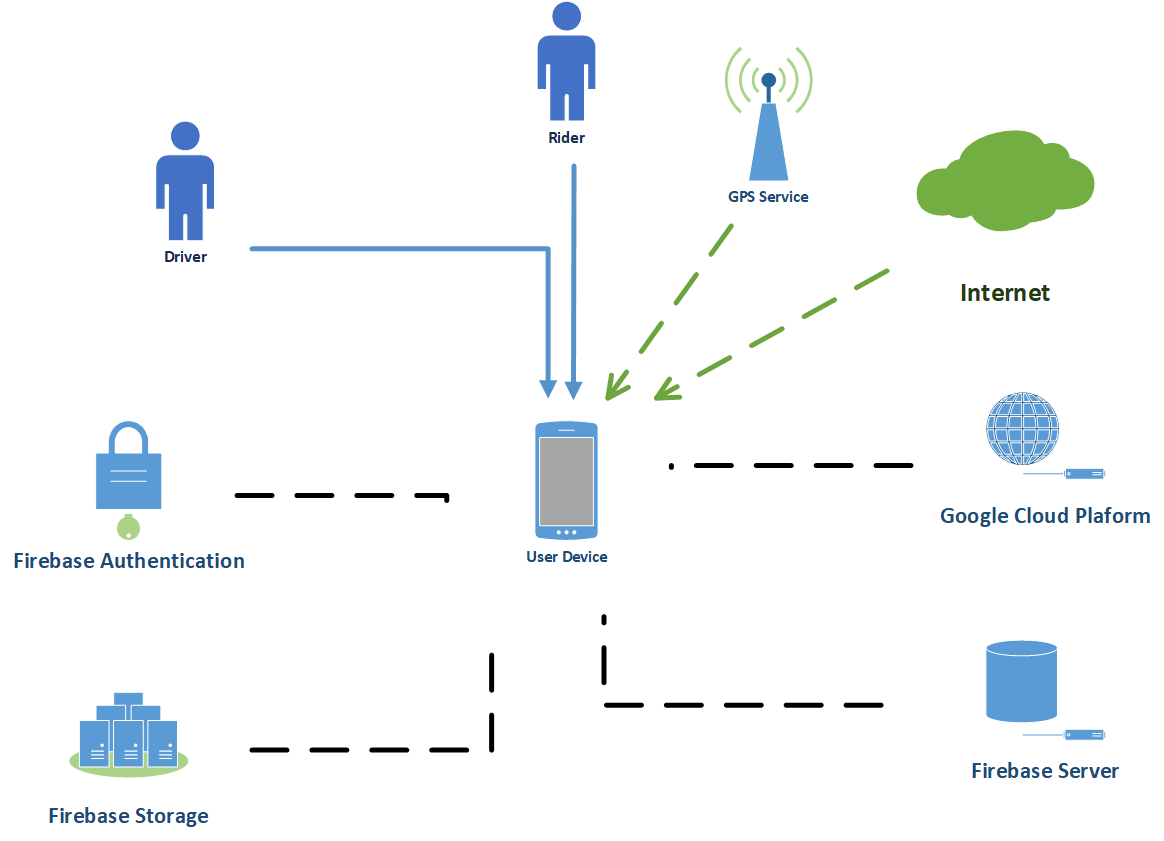
\includegraphics[width=0.8\textwidth]{SystemArchitectureCH5}
\caption{System Architecture}
\label{fig:System Architecture}
\end{figure}

\section{Work Environment}

\subsection{Hardware platforms}
For the development of this, application we have used an Hp Elitebook workstation 8460w. It is fairly powerful and could handle the usage of multiple emulators at once. The specifications of the machine are as follow:

\begin{itemize}
\item \textbf{Processor} : Intel® Core™ i7-2630QM Processor (2.0 GHz, 6 MB L3 Cache)
\item \textbf{Memory }: 12GB 1333 MHz DDR3 SDRAM (2D)
\item \textbf{Graphics }: AMD FirePro™ M3900 w/1 GB gDDR3
\item \textbf{HDD Drive }: 1TB
\end{itemize}

For the testing of the application on a real device, we have used Samsung Galaxy Note 8 and Huawei Mate 10 Pro.

\subsection{Software platforms}
As for the software part of the work environment, we have used several tools and frameworks alongside different versions of android.

\subsection{Work Tools}
\begin{itemize}
\item \textbf{Operating System }: Windows 
\item \textbf{IDE }: Android Studio 3.2.1
\item \textbf{Emulators }: Pixel 3 Android 9 / Nexus 5 Android 6
\item \textbf{Real Device OS}: Android 9 Pie (Samsung Galaxy Note 8)
\item \textbf{Backend Management}: Firebase Platform
\item \textbf{Places and Map Tools}: Google Cloud Platform
\end{itemize}
 

\subsection{Programming languages:} 
\begin{itemize}
\item \textbf{Application Programming }: Java\\

Motivation: Java code is inherently safer than Kotlin code because it prevents common programming mistakes by design, resulting in fewer system failures and application crashes.
\item \textbf{Layout Design }: XML
\item \textbf{Database Language }: NoSQL
\end{itemize}

\subsection{Frameworks used:}
\begin{itemize}
\item \textbf{Firebase Auth }: This framework lets you implement easy authentication. In this application, email and phone number authentication was used.
\item \textbf{Firebase Real-time Database }: This framework is used as our main database for this application. It lets you read and write data from firebase in a NoSQL structure. 
\item \textbf{Firebase Storage }: This framework is used to upload and download data such as photos and videos. This is used to store user pictures for our application.
\item \textbf{Firebase Messaging }: This framework makes real time messaging easy and possible using firebase. It is also used for push notifications which is used for messaging function between users in our application. 
\item \textbf{ Google Maps API }: This API enables the application to show places on the map like the origin and destination and the way between them. It is used in the map to trace the destination for users.
\item \textbf{Google Places API }: This API is used to give information about places in the application and used to AutoComplete search queries. It is used to auto complete search queries for our users for easier searching. It is also used to optimize our search function.
\item \textbf{Material Design Library }: This library provides components such as material buttons, material EditText etc.
\item \textbf{RuntimePermission }: This library helps to manage android permissions with no problems. 
\item \textbf{DxLoadingButton }: This library provides a loading button used for authentication. 
\item \textbf{Spinner }: Spinner is a styleable drop down menu for android using the old spinner style. 
\item \textbf{Tooltip }: Tooltip is a simple to use customizable library based on popup window. 
\item \textbf{EasyValidation }: EasyValidation is a text and input validation library in Java for android. It is used to validate user input information.
\item \textbf{Retrofit }: Retrofit is type-safe HTTP for Android and Java.
\end{itemize}

\section{Database Management System}
To manage the backend of our application we decided to use Firebase real-time database alongside with Firebase Auth and Firebase Storage. 
\begin{itemize}
\item \textbf{Firebase Real-time Database }\\

Its a NoSQL database. It's usage is very easy and very fast. We have used this database to store user objects which contain all the information about the users such as name, email, number etc. We have also used it to store trip and trip request objects.

\end{itemize}
\begin{figure}[ht]
\center
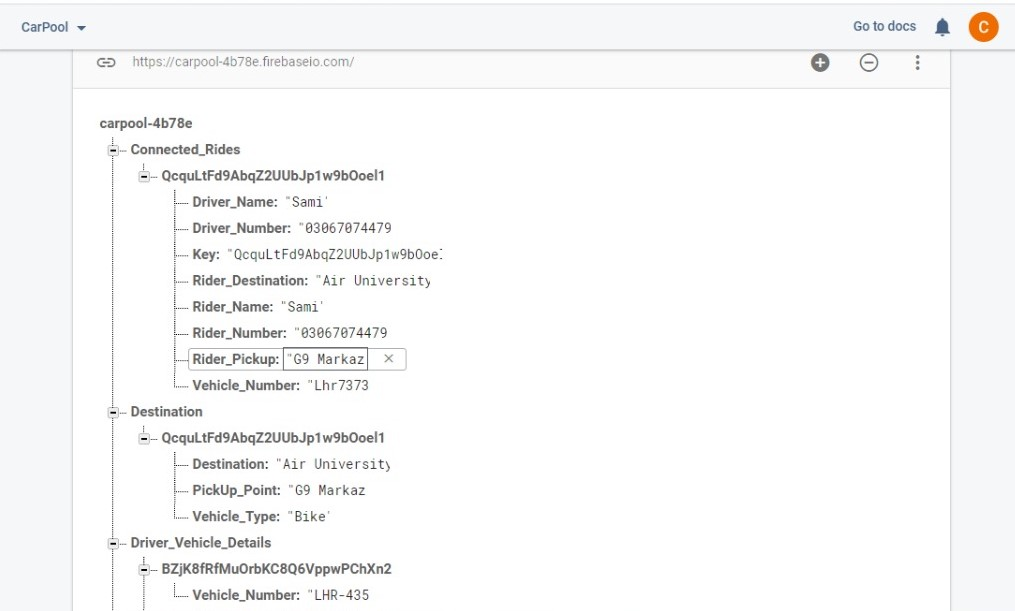
\includegraphics[width=1.0\textwidth]{DB-1} 
\caption{Example of a user mode in database}
\label{fig:Example of a user mode in database}
\end{figure}
\begin{figure}[ht]
\center
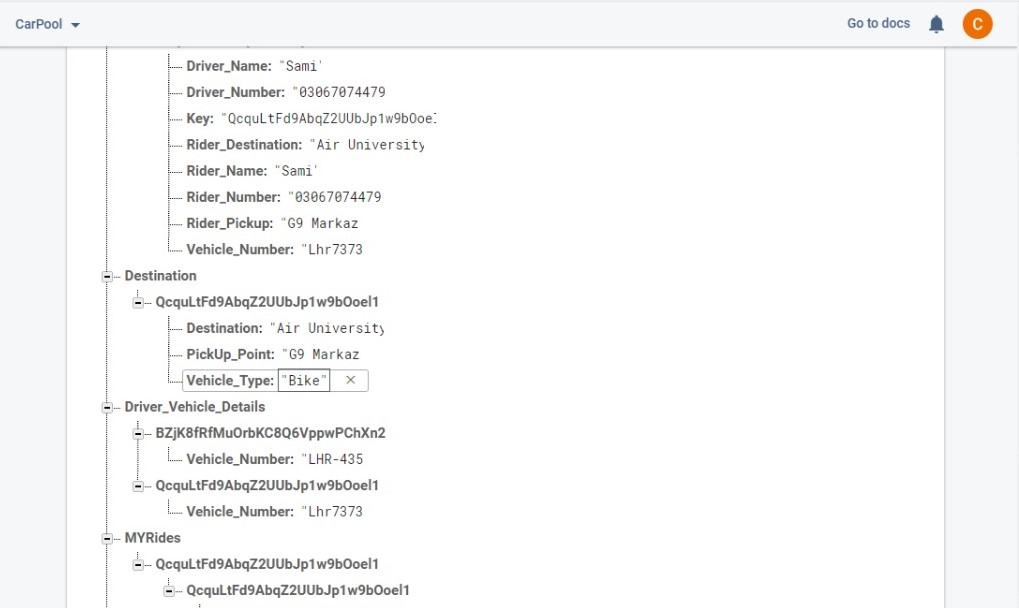
\includegraphics[width=1.0\textwidth]{DB-2} 
\caption{Example of a user mode in database}
\label{fig:Example of a user mode in database}
\end{figure}
\begin{itemize}
	
\item \textbf{Real-time Database Usage }\\

For the usage of this database, we made a separate database class. This class contains all database related functions with a listener interface. The reason for creating a separate class with a listener interface is to make migration to another database easier. If we ever decide to switch to another database, we will only change the content of the database class which would make changes faster, more professional and effective.\\

Firebase's real-time database allows you to use different query methods to fetch data. The first method is using \textbf{addListenerForSingleValueEvent}. This method listens to changes 
in data for one time and does not trigger until it’s called again. This is good for fetching data only once. The second method is using \textbf{addValueEventListener}. This method listens to data changes and is good for things like messages and real time updates.\\

We have decided to use \textbf{addListenerForSingleValueEvent} for most of our data fetching. The reason is each time data has been read, Firebase charges for it, which means if less data is fetched, the better it is in terms of cost. For this, we have avoided using \textbf{ addValueEventListener} and instead we fetch the data once and save it locally. When the data is changed, the user is required to refresh the page to get updates. However, in cases where it is important to get updates in real time like in messages, we have used \textbf{addValueEventListener}.
 
\end{itemize}

\section{Tools and Technology}
\begin{itemize}
\item Android
\item Firebase Platform
\item Google Cloud Platform
\item Android Studio
\item Java Language
\item Google Maps API
\item Google Direction API
\item Google Places API
\end{itemize}

\section{System requirements}
\begin{itemize}
\item Android phone with Minimum SDK android API 19 Kit Kat 
\item Google Play Services
\item GPS service
\item Internet Connection
\end{itemize}

\section{Security}
\begin{itemize}
\item \textbf{Firebase Authentication}\\ 

Firebase authentication is a very fast and secure way to sign users into our application. It is used to log in and register users into our database. In our case we are using the email verification. A user must verify his/her email to complete the registration.

\item \textbf{Authentication Usage}\\

When a user registers, his basic information (Name, Email, Password) are stored in the Auth database but not the real time Database. After that, users are welcomed with a finish registration activity. In this activity, they have to verify their email using EMAIL verification. This method is used to prevent spam and multiple account creations. After verification and filling other information, user data is saved on the real time database. 
\end{itemize}

\section{Rules}
Some of the restriction and rules are mentioned below :
\begin{itemize}
\item Users can use one account for both driver and rider.
\item Users cannot modify anyone else's data except theirs.
\item Only the admin can modify the data of other users.
\item The driver cannot select more than three riders.
\item The rider can only contact with their driver.
\item A rider has to select pick up and drop off points.
\item Driver and rider cannot use the app until their accounts are verified.
\end{itemize}
